\begin{frame}{Assignment Problem}
\begin{figure}
    \centering
    \includegraphics[height=5cm]{img/introduction/assignment.png}
\end{figure}
\end{frame}

\begin{frame}
	\centering \textbf{\huge Definitions}
\end{frame}


\begin{frame}[t]{Matching}
  \begin{block}{Definition}
    Set of non overlapping edges.
  \end{block} 

  \vspace{1em}
  \begin{figure}
    \centering
    \includegraphics[width=.25\linewidth]{img/introduction/graph01.eps}
    \hspace{2em}	
    \includegraphics[width=.25\linewidth]{img/introduction/graph02.eps}
  \end{figure}	
\end{frame}

\begin{frame}[t]{Bipartite Matching}
  \begin{block}{Definition}
  	Matching on a bipartite graph.
  \end{block} 
	
  \vspace{1em}
  \begin{figure}
	\centering
	\includegraphics[width=.25\linewidth]{img/introduction/bipar.eps}
	\hspace{3em}	
	\includegraphics[width=.25\linewidth]{img/introduction/biparmatch.eps}
  \end{figure}
\end{frame}

\begin{frame}[t]{Perfect Matching}
	\begin{block}{Definition}
	  Matching of size $\frac{|V\left(G\right)|}{2}$.
	\end{block} 
	
	\vspace{1em}
	\begin{figure}
	  \centering
	  \includegraphics[width=0.3\linewidth]{img/introduction/perfectmatching.eps}
	\end{figure}	
\end{frame}

\begin{frame}[t]{Maximum Matching}
	\begin{block}{Definition}
      Matching of the maximum size.
	\end{block} 
	
	\vspace{1em}
	\begin{figure}
		\centering
		\includegraphics[width=0.3\linewidth]{img/introduction/perfectmatching.eps}
	\end{figure}	
\end{frame}

\begin{frame}[t]{Maximum Matching vs Maximal Matching}
	Maximum: matching of the maximum size:
	\begin{center}
		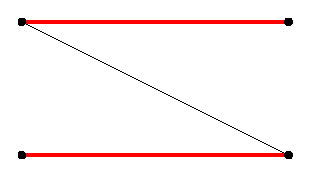
\includegraphics[width=0.35\linewidth]{img/introduction/maximummatching.eps}
	\end{center}

	Maximal: no more edges can be added:
	\begin{center}
  	\includegraphics[width=0.35\linewidth]{img/introduction/maximalmatch.eps}
	\end{center}
\end{frame}
